\section{Validation objective and scope}

This case asks whether ELMFIRE, driven by LANDFIRE fuels and terrain, hourly
analyzed weather and the observed ignition points, reproduces the hourly growth
of the \FireName{} (\FireYear{}) recorded by the GOES-Observed Fire Event
Representation (GOFER) product.  The comparison spans \DurationHours{}~h, from
the first GOES fire detection at \EventStart{} to the last GOFER perimeter at
\EventEnd{}.  The prediction quantity is the ELMFIRE fire arrival time on the
model grid; the reference quantity is the arrival time implied by the GOFER
hourly perimeters.  The case exercises the coupled surface-fire, crown-fire,
firebrand-spotting and level-set spread processes of ELMFIRE.  It does not
isolate any single algorithm, and it does not represent fire suppression,
which strongly affected the late growth of most of these fires.

The question is two-sided: does the simulated footprint reach the observed
burned area, and does it do so without excessive growth outside it?  Overlap,
omission, commission, area and arrival-time error are therefore reported
together, at fixed times after ignition.  No independent, predeclared
acceptance thresholds exist for this fire, so results are
\emph{characterized}; they are not labeled PASS or FAIL.  \CalibrationNote{}

\section{Reference event, experiment, and observations}

\FireSummary{}  GOFER derives hourly fire perimeters from the active-fire
detections of the GOES-East and GOES-West geostationary satellites
\cite{liu2024gofer,liu2023goferdata}.  For each hour the maximum detection
confidence of each satellite over the roughly 10-minute full-disk images is
combined, corrected for terrain parallax, smoothed, thresholded and vectorized
into a cumulative perimeter.  The combined product used here has an
area-weighted grid resolution of about 1.7~km.  Against California Fire and
Resource Assessment Program final perimeters for the 28 fires of the dataset,
the combined product reports a mean intersection over union of 0.77 and a mean
perimeter-position error of $0.75\pm0.21$~km \cite{liu2024gofer}.

The observation used for comparison is an arrival-time raster in which each
cell holds the first hour, measured from the GOES ignition hour, at which it
lies inside a cumulative GOFER perimeter.  It was produced by rasterizing the
\InputMetric{obs_hourly_perimeters} hourly perimeters of this fire on a
\InputMetric{obs_cell_size_m}-m grid in \CRSName{}.  The raster covers
\InputMetric{obs_burned_area_km2}~km$^2$, consistent with the final GOFER
perimeter area of \InputMetric{obs_gofer_final_area_km2}~km$^2$; arrival times
range from \InputMetric{obs_first_arrival_h} to
\InputMetric{obs_last_arrival_h}~h.  Because the satellite pixels are about
2~km across, the observed arrival time is uncertain by roughly one hour and the
footprint edge by several hundred meters, and growth below the detection limit
of GOES is not recorded.  The early perimeters of GOFER are scaled to account
for small fires that are not resolved \cite{liu2024gofer}.  These limitations
apply equally to every simulation compared here.

\begin{figure}[H]
  \centering
  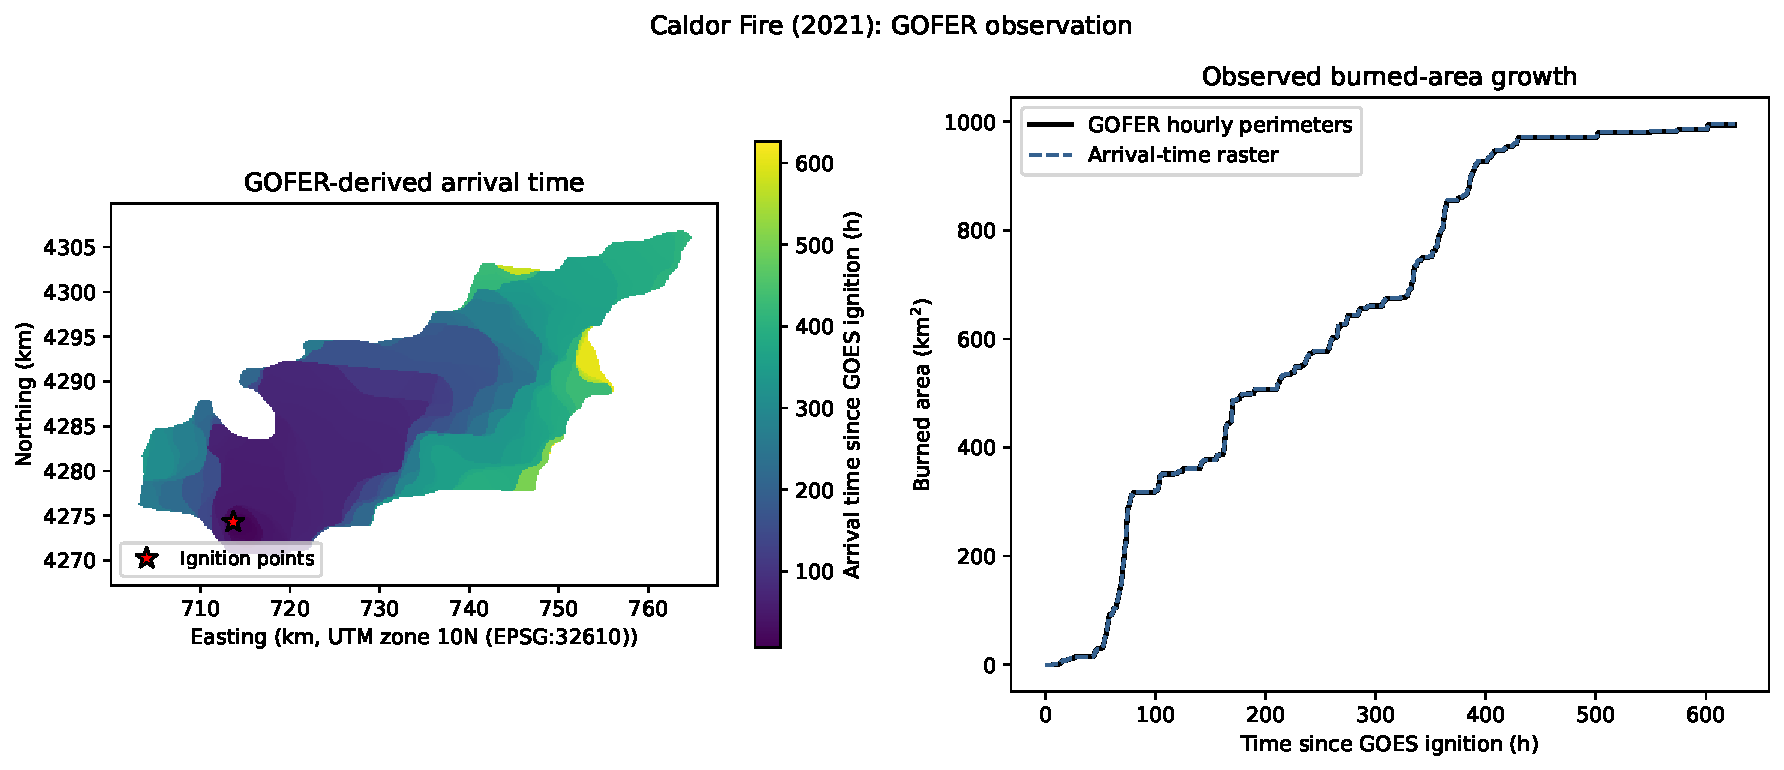
\includegraphics[width=0.98\textwidth,height=0.4\textheight,keepaspectratio]{observation_summary.pdf}
  \caption{GOFER observation of the \FireName{}: arrival time derived from the
  hourly perimeters (left; hours since the GOES ignition hour, \CRSName{}) and
  observed burned-area growth from the hourly perimeters and from the
  arrival-time raster (right).  Stars mark the GOFER ignition points.}
\end{figure}

\section{Input data provenance and characterization}

\begin{table}[H]
\centering{\small
\begin{tabular}{@{}p{0.2\textwidth}p{0.36\textwidth}p{0.36\textwidth}@{}}
\toprule
Input & Source and version & Resolution, units and processing \\
\midrule
Terrain & LANDFIRE elevation, slope and aspect \cite{landfire} & 30~m; m and degrees; \CRSName{} \\
Surface fuels & LANDFIRE 40 Scott and Burgan fuel models \cite{scott2005,landfire}, \FuelVersionText{} & 30~m categorical \\
Canopy & LANDFIRE canopy cover, height, base height and bulk density, \FuelVersionText{} & 30~m; percent, m, m and kg~m$^{-3}$ \\
Weather & Real-Time Mesoscale Analysis (RTMA) \cite{depondeca2011rtma}, retrieved as hourly fields through the CloudFire service \cite{cloudfire} & 600~m hourly; 20-ft wind speed in mph, direction the wind blows from in degrees \\
Fuel moisture & Dead (1-, 10- and 100-h) and live (herbaceous and woody) moisture derived by CloudFire from the analyzed weather & 600~m hourly; percent; derivation method not documented in the available case materials \\
Ignition & GOFER ignition points \cite{liu2023goferdata} & Points with hourly time stamps \\
Adjustment and initial state & Spread-rate adjustment factor and initial level set & Uniform value of one (no adjustment, nothing burned at the start) \\
\bottomrule
\end{tabular}}
\caption{Provenance of the model inputs.  Fuels, terrain and weather were
retrieved on 20 October 2026 for a domain centered on the GOFER perimeter.}
\end{table}
\ReportBodyText

The model domain is \InputMetric{grid_width} by \InputMetric{grid_height} cells
of \InputMetric{grid_cell_size_m}~m (\InputMetric{grid_area_km2}~km$^2$) in
\CRSName{}, extending 10~km beyond the bounding box of the final GOFER
perimeter.  Elevation ranges from \InputMetric{dem_minimum} to
\InputMetric{dem_maximum}~m (median \InputMetric{dem_median}~m) and slope has a
median of \InputMetric{slp_median}$^\circ$ and a 95th percentile of
\InputMetric{slp_p95}$^\circ$; the circular-mean aspect is
\InputMetric{asp_circular_mean}$^\circ$.  By area the domain is
\InputMetric{fuel_grass}\% grass, \InputMetric{fuel_grass_shrub}\% grass-shrub,
\InputMetric{fuel_shrub}\% shrub, \InputMetric{fuel_timber_understory}\%
timber-understory, \InputMetric{fuel_timber_litter}\% timber litter,
\InputMetric{fuel_slash_blowdown}\% slash-blowdown and
\InputMetric{fuel_non_burnable}\% non-burnable fuel models.  Canopy cover has a
median of \InputMetric{cc_median}\% and canopy base height a median of
\InputMetric{cbh_median}~m.  \OffshoreNote{}

\begin{figure}[H]
  \centering
  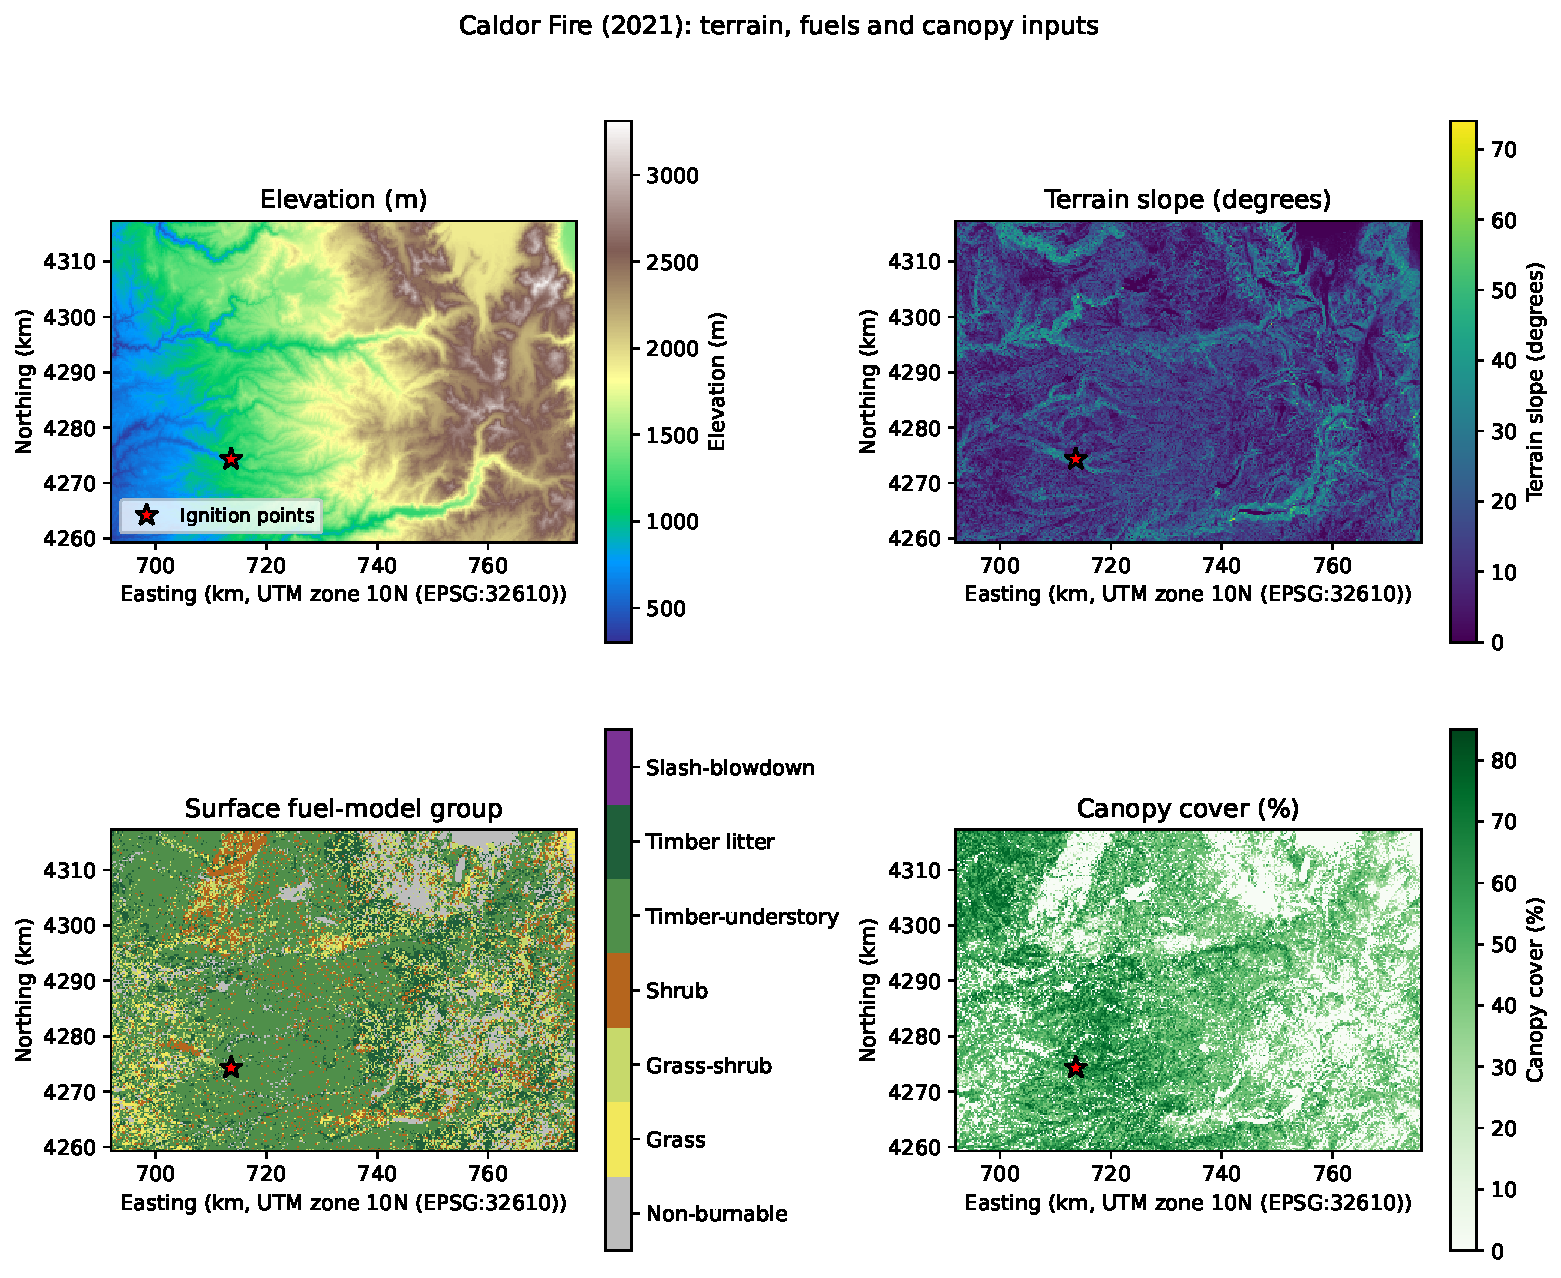
\includegraphics[width=0.9\textwidth,height=0.5\textheight,keepaspectratio]{input_overview.pdf}
  \caption{Model inputs over the whole domain: elevation, terrain slope,
  surface fuel-model group and canopy cover on the 30-m grid (\CRSName{}).
  Stars mark the ignition points.  These fields characterize model forcing;
  they are not validation evidence.}
\end{figure}

\begin{figure}[H]
  \centering
  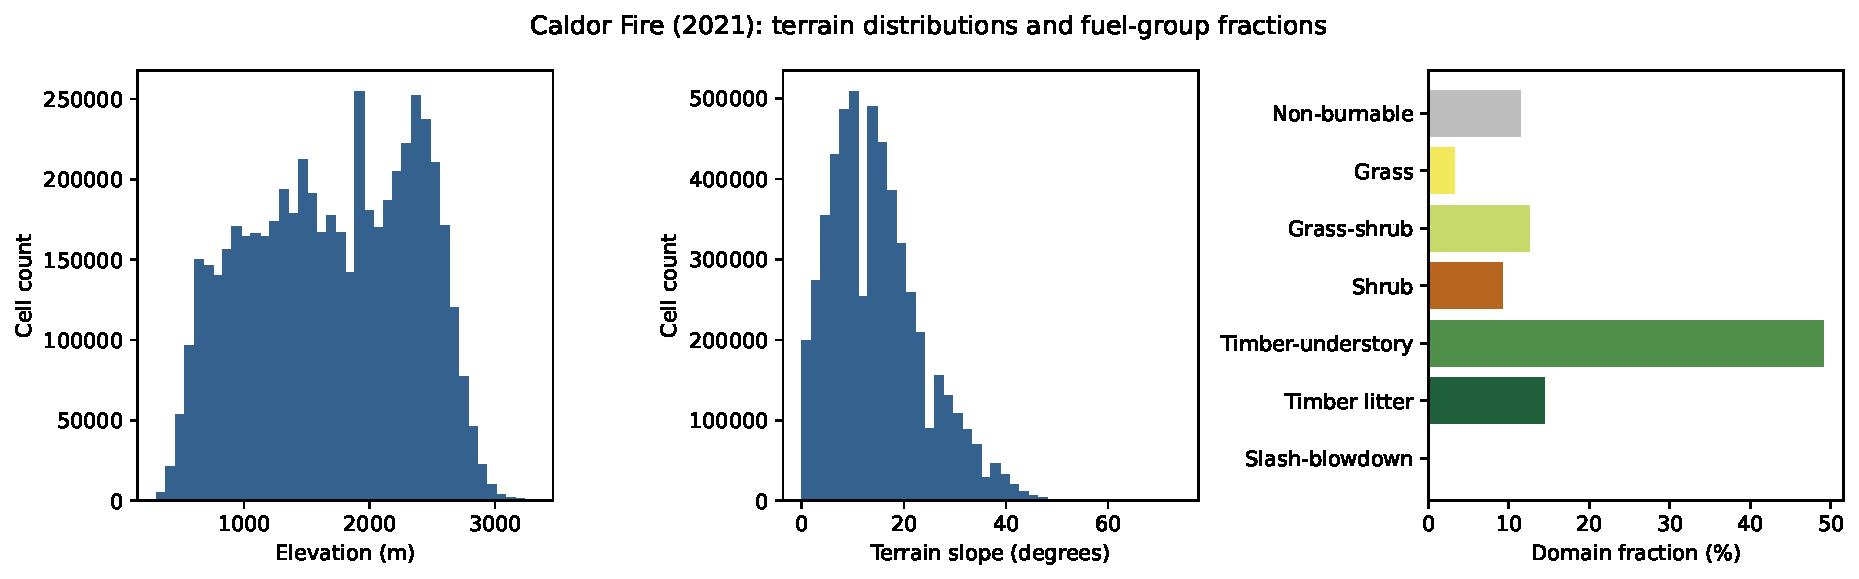
\includegraphics[width=0.98\textwidth,height=0.3\textheight,keepaspectratio]{input_distributions.pdf}
  \caption{Distributions of elevation and terrain slope over valid cells, and
  fraction of the domain in each surface fuel-model group.}
\end{figure}

The weather comprises \InputMetric{weather_bands} hourly fields.  Over all
hours and cells the 20-ft wind speed has a median of \InputMetric{ws_median}~mph
and a 95th percentile of \InputMetric{ws_p95}~mph; the circular-mean
direction the wind blows from is \InputMetric{wd_circular_mean}$^\circ$ with a
mean resultant length of \InputMetric{wd_resultant} (one for a constant
direction, zero for uniformly spread directions).  The 1-h dead-fuel moisture
has a median of \InputMetric{m1_median}\% (5th percentile
\InputMetric{m1_p05}\%), and live herbaceous and woody moisture have medians of
\InputMetric{lh_median}\% and \InputMetric{lw_median}\%.  Pooled values hide the
evolution of the event, so domain summaries are also shown by hour.

\begin{figure}[H]
  \centering
  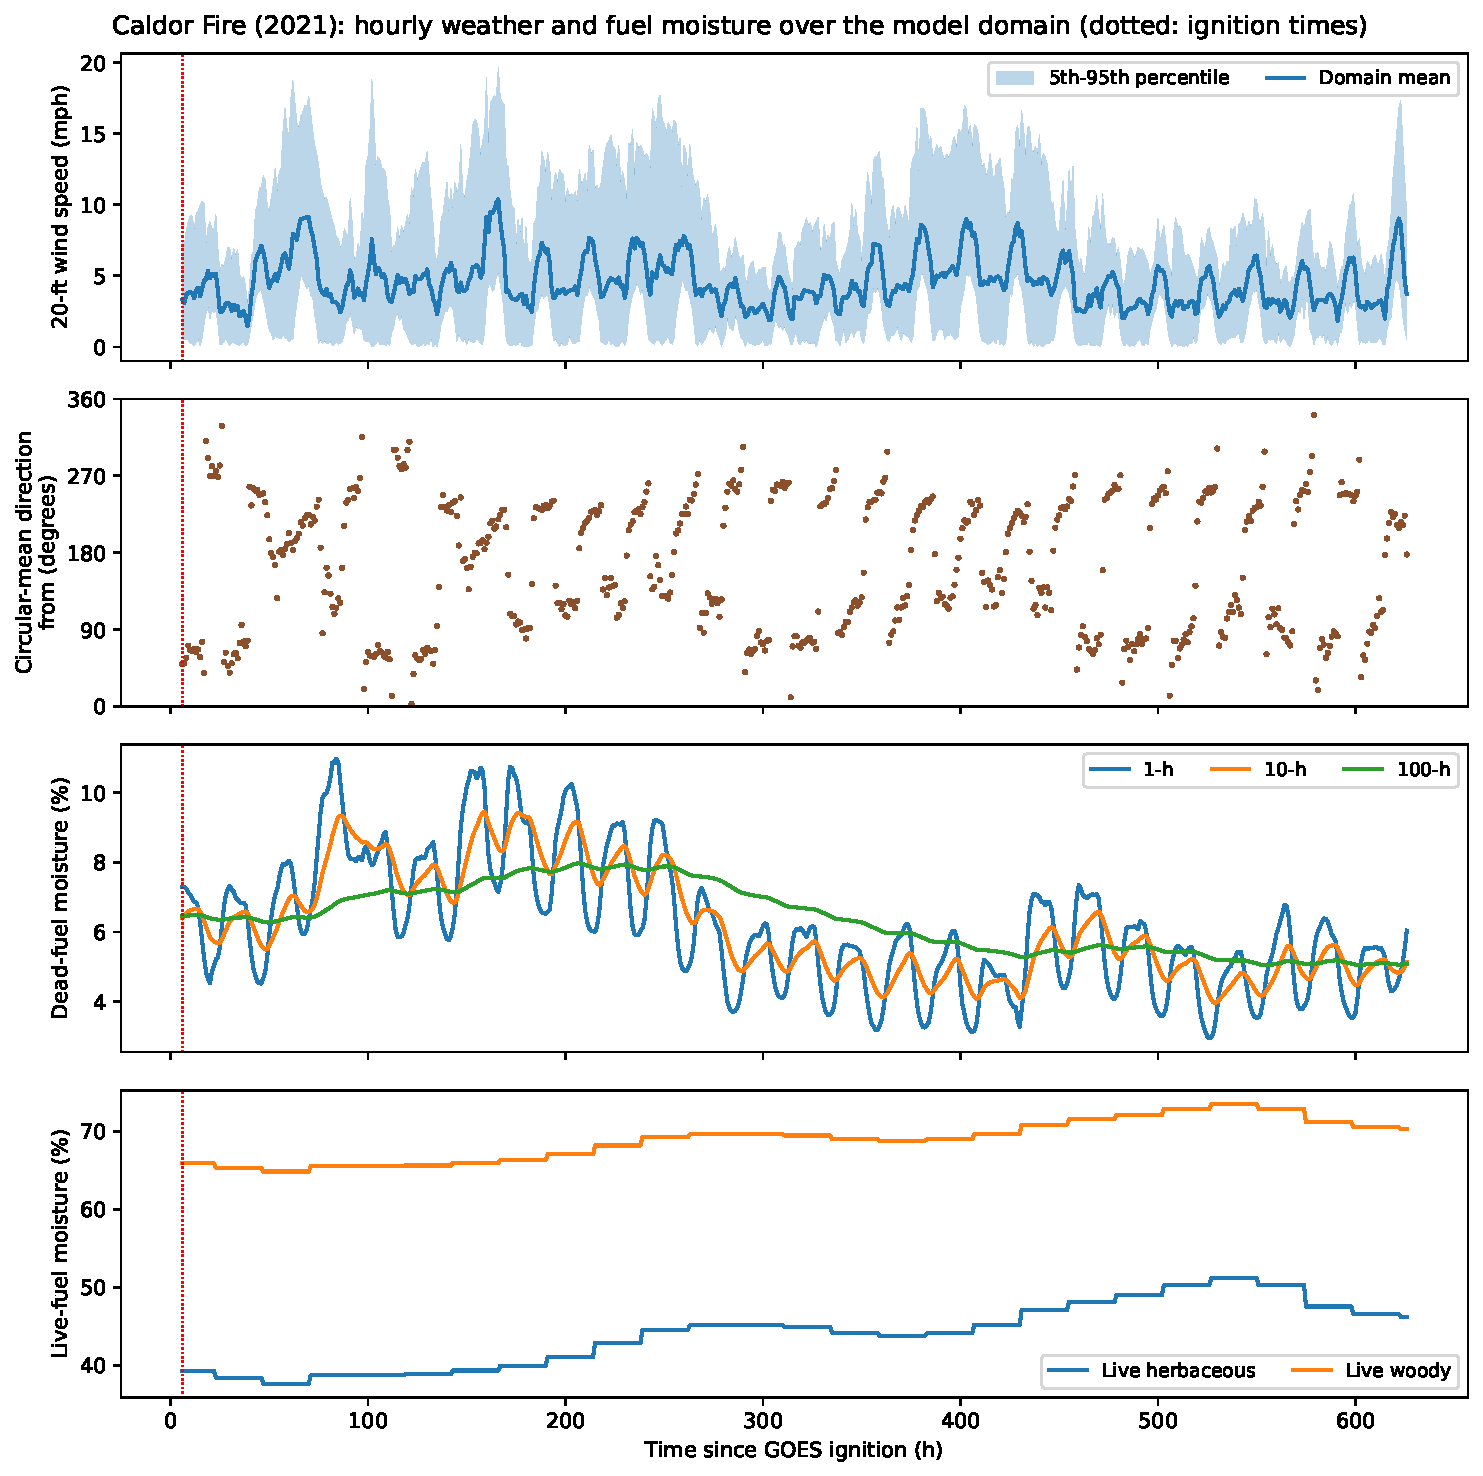
\includegraphics[width=0.95\textwidth,height=0.5\textheight,keepaspectratio]{weather_time_series.pdf}
  \caption{Hourly weather and fuel moisture over the model domain, in hours
  since the GOES ignition hour: domain-mean 20-ft wind speed with its 5th--95th
  percentile range, circular-mean wind direction (direction the wind blows
  from), and domain-mean dead- and live-fuel moisture.  Dotted lines mark the
  ignition times.}
\end{figure}

\begin{figure}[H]
  \centering
  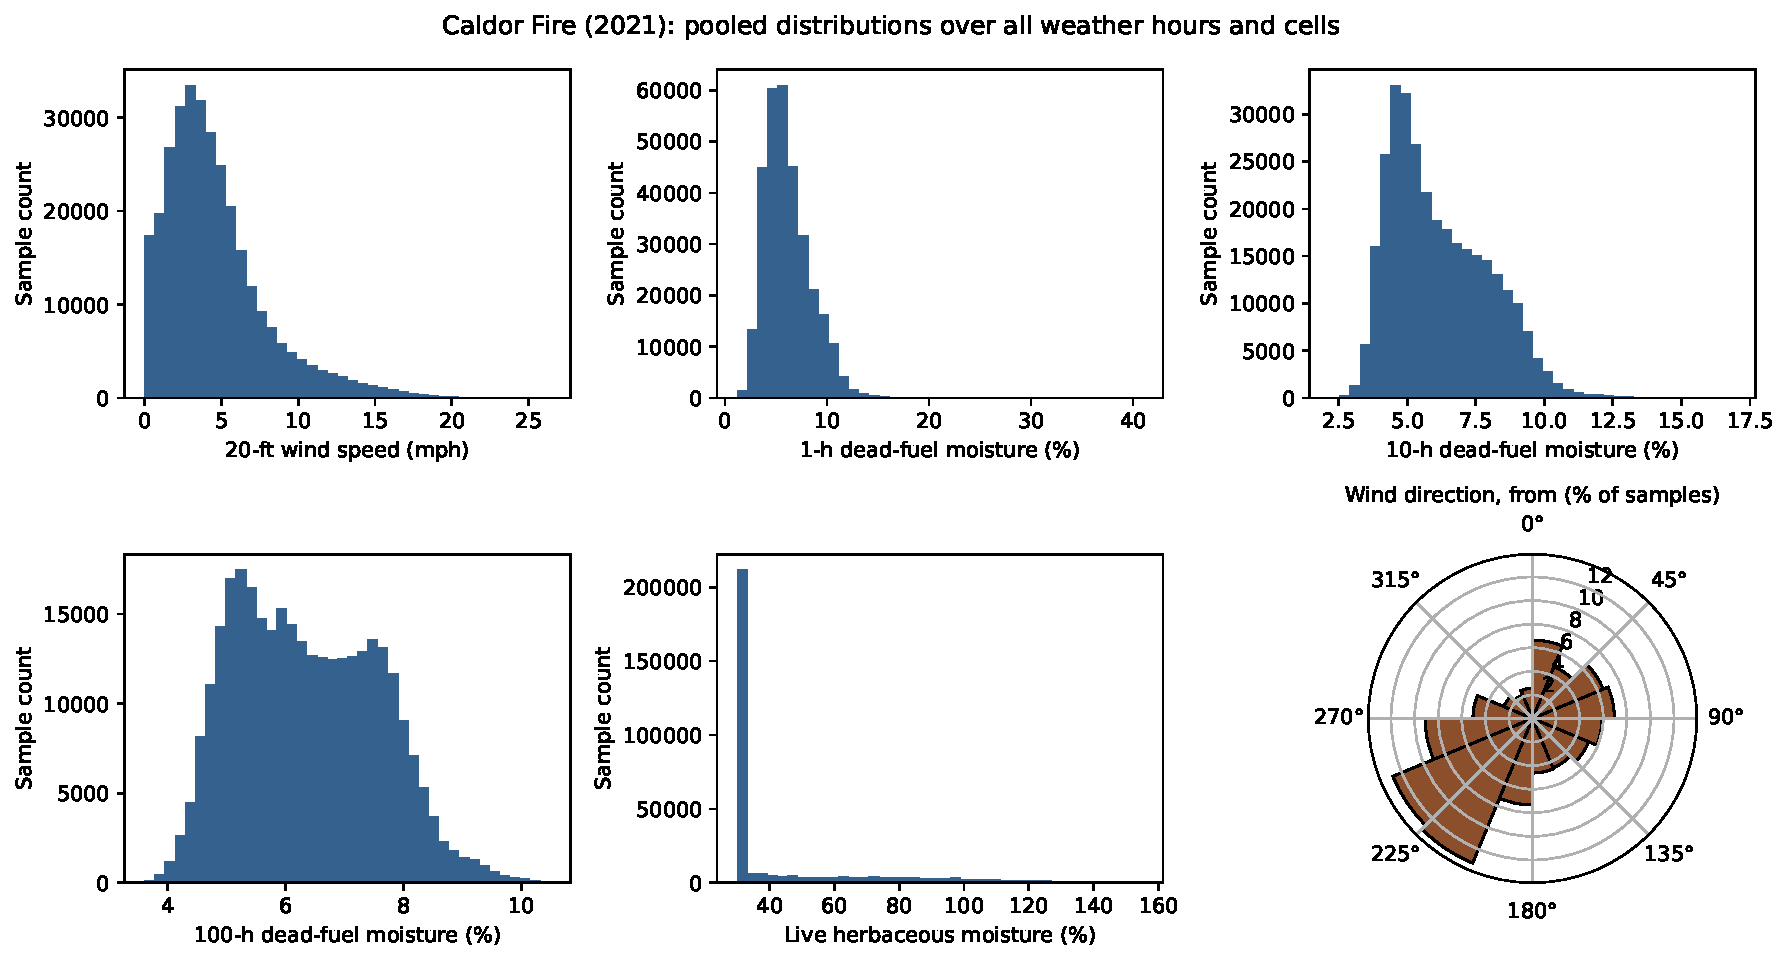
\includegraphics[width=0.95\textwidth,height=0.42\textheight,keepaspectratio]{weather_summary.pdf}
  \caption{Pooled distributions of wind speed and fuel moisture over all hours
  and a deterministic regular sample of cells, and the wind-direction rose
  (fraction of samples by the direction the wind blows from).}
\end{figure}

\section{Model configuration and rationale}

\ConfigurationText{}

\begin{table}[H]
\centering{\small
\begin{tabular}{@{}p{0.3\textwidth}p{0.2\textwidth}p{0.42\textwidth}@{}}
\toprule
Choice & Basis & Evidence and limitation \\
\midrule
Ignition points and times & documented & GOFER ignition record; \IgnitionMoveNote{} \\
Simulation start and stop & documented & First GOFER ignition point and last GOFER perimeter \\
Fuel vintage & derived & Latest LANDFIRE release whose mapped disturbances end before the fire year, so the fuels do not contain this fire \\
Weather and moisture & user-specified & RTMA analysis through CloudFire, as stated by the case owner \\
Crown fire & documented & ELMFIRE default crown-fire treatment, set explicitly \\
Firebrand spotting & user-specified & Enabled with ELMFIRE default spotting settings until calibration \\
Domain margin & user-specified & 10~km beyond the final GOFER perimeter \\
Single deterministic member & user-specified & No ensemble; stochastic spotting uses a fixed random seed \\
\bottomrule
\end{tabular}}
\caption{Basis of consequential configuration choices.}
\end{table}
\ReportBodyText

\section{Preprocessing and reproducibility}

Fuels, terrain and weather were retrieved through the CloudFire service for a
rectangular domain centered on the bounding box of the final GOFER perimeter.
The eight terrain, fuel and canopy layers were stacked into one landscape
raster without resampling.  Offshore cells outside LANDFIRE coverage, delivered
with a fill value that is not the declared missing-data value, were assigned
LANDFIRE's own open-water values (non-burnable fuel, zero elevation, slope and
canopy).  Each GOFER ignition point was projected to \CRSName{}; a point on a
non-burnable cell was moved to the nearest burnable cell within 300~m.
Simulation time starts at the first ignition hour, \WeatherOffsetText{}

The provided inputs are checked before analysis: required files must be
present with the recorded sizes, the landscape must have eight bands in the
recorded coordinate reference system and no unfilled cells, and every weather
field must cover the landscape with the recorded number of hourly bands.  The
input statistics and figures are then regenerated.  Large inputs and
simulation results are supplied to the case rather than stored in it; the
source record identifies each file, its size and its role.  \RevisionText{}

\section{Validation metrics and comparison method}

Let $\tau_s(\mathbf{x})$ be the simulated and $\tau_o(\mathbf{x})$ the GOFER
arrival time of cell $\mathbf{x}$, both in hours since the GOES ignition hour.
The simulated arrival time is the time-of-arrival output of the single
simulation member at its final output time, shifted by the offset between the
simulation start and the GOES ignition hour; unburned cells have no arrival
time.  The GOFER raster is transferred to the 30-m model grid by
nearest-neighbor sampling, so observed times are never interpolated, and the
comparison region is every valid landscape cell.  At comparison time $t$ the
footprints are $S_t=\{\mathbf{x}:\tau_s\le t\}$ and $O_t=\{\mathbf{x}:\tau_o\le
t\}$, and with $I_t=|S_t\cap O_t|$,
\begin{align}
 J_t&=\frac{I_t}{|S_t\cup O_t|}, &
 P_t&=\frac{I_t}{|S_t|}, &
 R_t&=\frac{I_t}{|O_t|}, &
 F_t&=\frac{2P_tR_t}{P_t+R_t}, &
 A_t&=\frac{|S_t|}{|O_t|}.
\end{align}
The Jaccard overlap $J_t$ summarizes footprint agreement; precision $P_t$
diagnoses commission (simulated burning outside the observation), recall $R_t$
omission (observed burning the simulation misses), $F_t$ balances the two, and
the area ratio $A_t$ exposes size compensation that overlap alone can hide.
The fixed comparison times are 24, 48 and 72~h and the last GOFER arrival time;
fixed times avoid choosing favorable instants, and the early times limit the
influence of suppression, which the model does not represent.  For cells burned
in both footprints by the final time, the arrival-time difference
$\tau_s-\tau_o$ is summarized by its mean (bias), median, mean absolute value
and root mean square.  Burned-area growth and hourly Jaccard overlap give the
time history.  The time at which the simulated fire first reaches the domain
boundary and whether propagation stalled before the planned end are reported
because both truncate simulated growth.

Results from different simulation configurations are evaluated separately and
never pooled.  A configuration is characterized when its time-of-arrival
result is available; a case with no simulation result is NOT EVALUABLE.
Because no acceptance threshold has been declared independently of these
results, no result is labeled PASS or FAIL.

\section{Simulation results and field-level comparison}

The current status of this case is \textbf{\Metric{status}}.  \Metric{reason}

\SimulationFields{}

\section{Integrated statistics and calculated metrics}

\IntegratedResults{}

\SimulationMetrics{}

\section{Interpretation and uncertainty}

Low overlap with high recall and low precision indicates overgrowth; high
precision with low recall indicates undergrowth or a displaced trajectory, and
an area ratio near one cannot by itself establish spatial agreement.  Late
comparison times are dominated by processes outside the model: suppression,
which stopped growth of the observed fire, and the finite model domain, which
stops simulated growth at its boundary.  The early comparison times are
therefore the most informative about spread physics.  \CaseInterpretation{}

The dominant uncertainties are the coarse spatial resolution of the satellite
observation and its hourly sampling, the 2.5-km resolution of the weather
analysis, which smooths local terrain-driven winds, the LANDFIRE fuel
classification, the undocumented derivation of fuel moisture, the ignition
location uncertainty of about one GOES pixel, and the default firebrand-spotting
parameters.  A single deterministic member does not quantify uncertainty;
model-form, parameter and input errors are not separable with these metrics
alone.

\section{Conclusions and limitations}

The case characterizes the agreement between ELMFIRE and the GOFER hourly
progression of the \FireName{}.  Inputs and the observation are characterized
in full; the current scientific status is \textbf{\Metric{status}} with
\Metric{simulations_found} simulation result(s) evaluated.  The results
describe the configurations listed and do not transfer to other
configurations, fires or weather products.  A defensible validation decision
requires acceptance thresholds fixed before the evaluated run, an ensemble that
represents weather, fuel and ignition uncertainty, documentation of the
fuel-moisture derivation, and evaluation of any calibrated parameters on fires
not used to choose them.

\begin{thebibliography}{9}
\bibitem{liu2024gofer} T.~Liu, J.~T. Randerson, Y.~Chen, D.~C. Morton, E.~B. Wiggins, P.~Smyth, E.~Foufoula-Georgiou, R.~Nadler and O.~Nevo, ``Systematically tracking the hourly progression of large wildfires using GOES satellite observations,'' \emph{Earth System Science Data}, 16, 1395--1424, 2024, \href{https://doi.org/10.5194/essd-16-1395-2024}{doi:10.5194/essd-16-1395-2024}.
\bibitem{liu2023goferdata} T.~Liu et al., GOFER product and algorithm for 28 California fires, 2019--2021, Zenodo, 2023, \href{https://doi.org/10.5281/zenodo.8327264}{doi:10.5281/zenodo.8327264}.
\bibitem{landfire} LANDFIRE, U.S. Department of the Interior, Geological Survey, and U.S. Department of Agriculture, \href{https://landfire.gov}{landfire.gov}.
\bibitem{scott2005} J.~H. Scott and R.~E. Burgan, ``Standard fire behavior fuel models: a comprehensive set for use with Rothermel's surface fire spread model,'' USDA Forest Service General Technical Report RMRS-GTR-153, 2005.
\bibitem{depondeca2011rtma} M.~S.~F.~V. De Pondeca et al., ``The Real-Time Mesoscale Analysis at NOAA's National Centers for Environmental Prediction: current status and development,'' \emph{Weather and Forecasting}, 26, 593--612, 2011.
\bibitem{cloudfire} C.~Lautenberger, ELMFIRE and the CloudFire fuel, weather and ignition data service, \href{https://elmfire.io}{elmfire.io}.
\bibitem{vanwagner1977} C.~E. Van Wagner, ``Conditions for the start and spread of crown fire,'' \emph{Canadian Journal of Forest Research}, 7, 23--34, 1977.
\bibitem{cruz2005} M.~G. Cruz, M.~E. Alexander and R.~H. Wakimoto, ``Development and testing of models for predicting crown fire rate of spread in conifer forest stands,'' \emph{Canadian Journal of Forest Research}, 35, 1626--1639, 2005.
\end{thebibliography}
